\section{Waves of nearly constant modulus}\label{sec:waves}

The balanced coefficients of Proposition~\ref{prop:balanced} allow us to
build a function on the circle whose modulus stays close to one.  Its
oscillations spread its Fourier mass over the indices $0,\ldots,N-1$.
The essential endpoint choice is to increase phase curvature, rather than
to decrease modulus: the resulting endpoint contributions are small while
the function remains bounded away from zero.

\begin{proposition}\label{prop:waves}
There are absolute constants $C>0$ and $\delta_0>0$ with the following
property.  For every $0<\delta<\delta_0$, there are $N_0(\delta)$ and
$K_\delta<\infty$ such that, for every integer $N\ge N_0(\delta)$, there is
a continuous function $B_N:\T\to\C$ satisfying
\begin{align}
 B_N(-t)&=\overline{B_N(t)}, &
 1\le |B_N(t)|&\le 1+C\delta \quad(t\in\T),
 \label{eq:wave-modulus}\\
 \sqrt N\,|\widehat B_N(k)|&\le 1+C\sqrt\delta
 &&(0\le k<N),\label{eq:wave-coefficients}\\
 \sum_{k<0\text{ or }k\ge N}|\widehat B_N(k)|
 &\le K_\delta N^{-1}.\label{eq:wave-tail}
\end{align}
Its Fourier coefficients are real, and its Fourier series converges
absolutely and represents $B_N$.
\end{proposition}

We use the following packing result from the preceding version.  Its
proof combines a finite-field construction with almost-perfect matchings
in nearly regular hypergraphs; only its stated conclusion is needed here.

\begin{lemma}[Signed interval packing, {\cite[Lemma~3.1]{OpenAILowerEnvelope2026}}]
\label{lem:signed-packing}
Let $a_1,\ldots,a_r\in\Z^m\setminus\{0\}$ be pairwise nonparallel, with
$r\ge2$, and let $w_1,\ldots,w_r>0$ satisfy $2\sum_iw_i<1$.
There are an integer $H\ge1$ and points $\theta_1,\ldots,\theta_H\in\T^m$
such that the closed arcs centered at $\pm a_i\cdot\theta_h$, of length
$w_i/H$, are pairwise disjoint as $i$, $h$, and the sign vary.
\end{lemma}

\begin{proof}[Proof of Proposition~\ref{prop:waves}]
Fix $\delta$ and choose the data of Proposition~\ref{prop:balanced}.
Thus
\[
 F(y)=\sum_{a\in\mathcal A}c_a\e(a\cdot y),\qquad
 \lambda_a=a\cdot v,\qquad w_a=|\lambda_a|,
\]
where $F$ is real, $\mathcal A=-\mathcal A$, and
\begin{equation}\label{eq:wave-input}
 \|F\|_\infty\le1+\delta,\qquad
 1-C\delta\le\sum_{a\in\mathcal A}w_a<1,\qquad
 1\le m_a:=\frac{|c_a|}{\sqrt{w_a}}\le1+C\delta\le2.
\end{equation}
There are at least two sign-pairs in $\mathcal A$, and representatives of
these pairs are nonparallel.  All choices below, apart from bounded phase
adjustments used to join endpoint values, will be fixed before $N$ tends
to infinity.  Constants depending on these choices are allowed in errors
that vanish with $N$; the constants multiplying $\delta$ and
$\sqrt\delta$ in the final bounds will be absolute.
We first obtain a bound $1+O(\delta)$ for the scaled Fourier contribution
of the main intervals, then fill their small complement at cost
$O(\sqrt\delta)$.  A separate integration-by-parts argument will control
the sum of the exterior coefficients.

\subsection*{Packed intervals and inverse curvature}

Apply Lemma~\ref{lem:signed-packing} to one representative from each
sign-pair, using $w_{-a}=w_a$.  It gives disjoint closed arcs centered at
$-a\cdot\theta_h$, of length $w_a/H$, for all $a\in\mathcal A$ and
$1\le h\le H$.  Each arc is disjoint from its reflection and consequently
avoids the two fixed points $0$ and $1/2$ of reflection on $\T$.
We may therefore regard the arcs as intervals in $(-1/2,1/2)$, with center
representatives $t^*_{a,h}$ satisfying
\begin{equation}\label{eq:wave-centers}
 t^*_{a,h}\equiv-a\cdot\theta_h\pmod1,\qquad
 t^*_{-a,h}=-t^*_{a,h}.
\end{equation}

The variable $x$ will denote the normalized Fourier index $k/N$.
For each $h$, choose a closed interval
\[
 J_h\subset((h-1)/H,h/H)
\]
symmetric about $x_h^*=(h-1/2)/H$.  On $J_h$ choose a smooth function
$\chi_h$, symmetric about $x_h^*$, such that
\begin{equation}\label{eq:wave-taper}
 \sigma\le\chi_h\le1,\qquad
 \chi_h=\sigma\text{ near both endpoints},\qquad
 \int_{J_h}\chi_h(x)^2\,dx\ge\frac{1-\delta}{H}.
\end{equation}
Here $\sigma\in(0,1)$ can be arbitrarily small.  Indeed, first choose
$|J_h|>(1-\delta/2)/H$, and then take $\chi_h=1$ except on endpoint
neighborhoods of total length less than $\delta/(2H)$, with smooth
transitions to $\sigma$.

We will specify the point $t$ at which a wave's phase derivative equals
$x$.  Requiring $|dt/dx|=w_a\chi_h(x)^2$ makes the stationary-phase
factor equal to $\sqrt{w_a}\chi_h(x)$, so a wave of modulus $m_a$ has
leading scaled coefficient magnitude $|c_a|\chi_h(x)$.  Thus $\chi_h$ can
suppress endpoint Fourier contributions without decreasing the wave
modulus.

Choose smooth real $Q_h$ with
\[
 Q_h''=\chi_h^2,\qquad Q_h'(x_h^*)=0,
\]
and with a smooth extension to a neighborhood of $J_h$.  Define
\begin{equation}\label{eq:wave-map}
 T_{a,h}(x)=t^*_{a,h}-\lambda_aQ_h'(x),\qquad x\in J_h.
\end{equation}
This is a diffeomorphism, possibly reversing orientation, onto a closed
interval $I_{a,h}$.  Symmetry and $\chi_h\le1$ give
$|Q_h'|\le |J_h|/2<1/(2H)$, so $I_{a,h}$ lies strictly inside its assigned
packed arc.  Write $X_{a,h}:I_{a,h}\to J_h$ for the inverse map and set
\begin{align}
 \psi_{a,h}(t)
 &= (t-t^*_{a,h})X_{a,h}(t)
       +\lambda_a Q_h(X_{a,h}(t)),\label{eq:wave-phase}\\
 \psi_{a,h}'(t)&=X_{a,h}(t),&
 \psi_{a,h}''(t)&=-\frac1{\lambda_a\chi_h(X_{a,h}(t))^2}.
 \label{eq:wave-phase-derivatives}
\end{align}
The derivative identities follow by differentiating
\eqref{eq:wave-phase} and using \eqref{eq:wave-map}.
On each $I_{a,h}$ define
\begin{equation}\label{eq:main-wave}
 B_N(t)=\frac{c_a}{\sqrt{w_a}}
 \e\bigl(\sgn(\lambda_a)/8+N\psi_{a,h}(t)\bigr).
\end{equation}
The modulus is the constant $m_a$.  Moreover,
$T_{-a,h}(x)=-T_{a,h}(x)$ and
$\psi_{-a,h}(-t)=-\psi_{a,h}(t)$; together with
$c_{-a}=\overline{c_a}$ these give conjugate symmetry on the main intervals.
Their total length is
\begin{equation}\label{eq:main-coverage}
 \sum_{a,h}|I_{a,h}|
 =\sum_{a,h}w_a\int_{J_h}\chi_h^2
 \ge(1-\delta)\sum_aw_a\ge1-C\delta.
\end{equation}

\subsection*{Coherent stationary contributions}

The phase choice will make the leading stationary contributions sum to a
scalar multiple of a single value of $F$.  We first isolate them with a
cutoff and estimate the remaining endpoint pieces using their large
curvature.

Choose $G_h\in C_c^\infty(\operatorname{int}J_h)$ with $0\le G_h\le1$,
such that, on $J_h$, $1-G_h$ is supported in the two endpoint intervals where
$\chi_h=\sigma$, and is monotone on each such interval.
Split each integral over $I_{a,h}$ using the cutoff
$G_h(X_{a,h}(t))$.  On either endpoint part the phase has constant second
derivative of modulus $1/(w_a\sigma^2)$.  The cutoff has bounded total
variation.  Lemma~\ref{lem:oscillatory-bounds} therefore bounds this part,
after multiplication by $\sqrt N$, by
\[
 C m_a\sqrt{w_a}\,\sigma=C|c_a|\sigma.
\]
Choose $\sigma$ so small, before fixing the functions in
\eqref{eq:wave-taper}, that the sum of these bounds over all endpoints is
at most $\delta$.

For the part with cutoff, apply Lemma~\ref{lem:stationary-phase} with
$x=k/N$.  After multiplication by $\sqrt N$, the leading term is zero
if $x\notin J_h$; if $x\in J_h$, its stationary point is
$t=T_{a,h}(x)$ and its value is
\begin{equation}\label{eq:main-leading-term}
 c_aG_h(x)\chi_h(x)
 \e\bigl(-kt^*_{a,h}+N\lambda_aQ_h(x)\bigr).
\end{equation}
Indeed,
\[
 \psi_{a,h}(T_{a,h}(x))-xT_{a,h}(x)
   =-xt^*_{a,h}+\lambda_aQ_h(x),
\]
and the phase correction $\sgn(\psi_{a,h}'')/8$ cancels the constant
$\sgn(\lambda_a)/8$ in \eqref{eq:main-wave}.
The error is $o(1)$ uniformly for $0\le k<N$.

At most one $J_h$ contains $x$.  For that $h$, summing
\eqref{eq:main-leading-term} over $a$ gives
\[
 G_h(x)\chi_h(x)F\bigl(k\theta_h+NvQ_h(x)\bigr).
\]
Here \eqref{eq:wave-centers} may be used inside the exponential because
$k$ is an integer.  Since $0\le G_h\chi_h\le1$, the norm bound for $F$
and the endpoint estimates imply
\begin{equation}\label{eq:main-fourier-bound}
 \sqrt N\left|\sum_{a,h}\int_{I_{a,h}}B_N(t)\e(-kt)\,dt\right|
 \le1+2\delta+o(1),\qquad 0\le k<N.
\end{equation}
All errors are uniform in these integer indices.  The finite number of
intervals is fixed, so summing their stationary-phase errors preserves
$o(1)$.

\subsection*{Joining the waves through the gaps}

It remains to define $B_N$ on a set of length $O(\delta)$ without losing
its lower modulus bound.  We will join the waves continuously and also
match the derivatives of their leading phases.  The first condition
preserves the desired function; together, the two conditions will cancel
the boundary terms in the exterior Fourier estimate.

Work first on $[0,1/2]$.  Let $[u_j,v_j]$ be the closures of the gaps
between its main intervals, including the gaps adjacent to $0$ and
$1/2$.  Put $l_j=v_j-u_j$ and $L=\sum_jl_j$.  Strict containment in the
packed arcs and \eqref{eq:main-coverage} give
\[
 0<L\le C\delta,
\]
and each $l_j$ is positive.  At an endpoint $z$ adjoining a main interval,
prescribe the derivative $x_z=\psi_{a,h}'(z)\in(0,1)$; at the remaining
endpoints prescribe $x_0=x_{1/2}=1/8$.

For each gap choose a closed interval $[P_j,R_j]\subset(1/4,3/4)$, of
length $l_j/(4L)$, such that these intervals are pairwise disjoint and
none of their endpoints equals any prescribed $x_z$.  To see that these
choices are possible, note that their total length is $1/4$.  They can
therefore be arranged with positive spaces between them inside an interval
of length less than $1/2$; a sufficiently small common translation then
avoids the finitely many forbidden endpoint values.  We call
$[P_j,R_j]$ the derivative interval assigned to gap $j$.

Divide gap $j$ into three pieces.  On these pieces take $\phi_j'$ to be
linear, successively interpolating
\begin{equation}\label{eq:gap-derivative-path}
 x_{u_j}\longrightarrow P_j\longrightarrow R_j\longrightarrow x_{v_j}.
\end{equation}
Thus $\phi_j$ is continuously differentiable and piecewise quadratic;
its additive constant is immaterial.  Make both outer pieces shorter
than $l_j/4$.  Their nonzero slopes $\Lambda=\phi_j''$ can be made
arbitrarily large in absolute value because $P_j\ne x_{u_j}$ and
$R_j\ne x_{v_j}$.  Choose their lengths so that
\begin{equation}\label{eq:gap-outer-slopes}
 \sum_{\substack{\text{outer pieces}\\\text{in }[0,1/2]}}
       |\Lambda|^{-1/2}\le\sqrt\delta.
\end{equation}
The middle piece has length at most $l_j$, so its positive slope satisfies
\begin{equation}\label{eq:gap-middle-slope}
 \Lambda\ge\frac{R_j-P_j}{l_j}=\frac1{4L}.
\end{equation}
Every value of every leading phase derivative lies in a fixed compact
subset of $(0,1)$.

Figure~\ref{fig:gap-derivative} illustrates the two distinct uses of these
pieces: large outer slopes suppress the cost of joining the prescribed
endpoint derivatives, while separated middle derivative intervals ensure
that only one middle pair can contribute substantially at a given
normalized Fourier index.

\begin{figure}[tb]
\centering
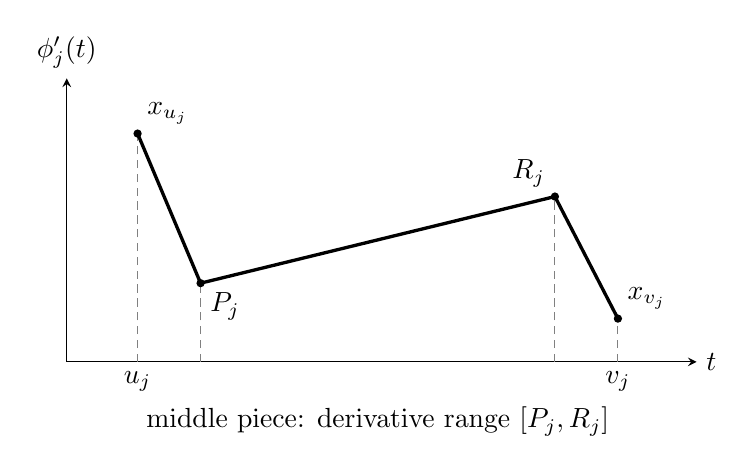
\begin{tikzpicture}[x=1cm,y=1cm,>=stealth]
 \draw[->] (0,0) -- (8,0) node[right] {$t$};
 \draw[->] (0,0) -- (0,3.6) node[above] {$\phi_j'(t)$};
 \draw[densely dashed,gray] (.9,0) -- (.9,2.9);
 \draw[densely dashed,gray] (1.7,0) -- (1.7,1.0);
 \draw[densely dashed,gray] (6.2,0) -- (6.2,2.1);
 \draw[densely dashed,gray] (7.0,0) -- (7.0,.55);
 \draw[very thick] (.9,2.9) -- (1.7,1.0) -- (6.2,2.1) -- (7.0,.55);
 \fill (.9,2.9) circle (1.5pt) node[above right] {$x_{u_j}$};
 \fill (1.7,1.0) circle (1.5pt) node[below right] {$P_j$};
 \fill (6.2,2.1) circle (1.5pt) node[above left] {$R_j$};
 \fill (7.0,.55) circle (1.5pt) node[above right] {$x_{v_j}$};
 \node[below] at (.9,0) {$u_j$};
 \node[below] at (7.0,0) {$v_j$};
 \node[below,align=center] at (3.95,-.45) {middle piece: derivative range $[P_j,R_j]$};
\end{tikzpicture}
\caption{A schematic leading phase derivative on one gap.  The short
outer pieces join the prescribed endpoint values to $P_j$ and $R_j$.
Their slopes may have either sign; the middle slope is positive.
The drawing shows one possible ordering of the endpoint values, and is
not to scale.}\label{fig:gap-derivative}
\end{figure}

Let $m_j$ interpolate linearly between the endpoint moduli $m_a$, with
modulus $1$ prescribed at $0$ and $1/2$.  Define on gap $j$
\begin{equation}\label{eq:gap-wave}
 B_N(t)=m_j(t)\e\bigl(N\phi_j(t)+\gamma_{j,N}(t)\bigr),
\end{equation}
where $\gamma_{j,N}$ is affine.  Choose its two endpoint values in
$[0,1)$ to give the exact phase factors required by the adjoining main
waves, and phase factor $1$ at $0$ and $1/2$.  There is no constraint on
these choices: each endpoint requires just one congruence modulo $1$.
In particular,
\[
 \int_{u_j}^{v_j}|\gamma_{j,N}'(t)|\,dt\le1,
 \qquad |\gamma_{j,N}'|\le l_j^{-1}.
\]
The second bound depends on the fixed gap but is independent of $N$.
Extend to the negative half-circle by
$B_N(-t)=\overline{B_N(t)}$.  Because $B_N(0)=B_N(1/2)=1$, this gives a
continuous function on $\T$ satisfying \eqref{eq:wave-modulus}.
On reflected gaps use the leading phase $-\phi_j(-t)$.  Its derivative is
$\phi_j'(-t)$, so the leading phase derivatives match across every join,
including $0$ and the identified endpoints $\pm1/2$.  Matching the full
derivatives of $B_N$ is unnecessary.

\subsection*{Fourier cost of the gaps}

We now bound the Fourier contributions of the gaps.  In
\eqref{eq:gap-wave} regard $f_N=m_j\e(\gamma_{j,N})$ as the amplitude.
On each piece,
\begin{equation}\label{eq:gap-amplitude-variation}
 \sup|f_N|+\int|f_N'|\le C
\end{equation}
with an absolute constant, since $m_j$ is monotone between values in
$[1,2]$ and the total variation of $\gamma_{j,N}$ is at most $1$.
Lemma~\ref{lem:oscillatory-bounds} and
\eqref{eq:gap-outer-slopes} show that all outer pieces and their
reflections contribute at most $C\sqrt\delta$ to the scaled Fourier
coefficient $\sqrt N\,\widehat B_N(k)$.

Choose a fixed $\rho>0$ so that the closed $\rho$-neighborhoods of the
finitely many derivative intervals $[P_j,R_j]$ are pairwise disjoint.
At most one of these intervals is within $\rho$ of $x=k/N$.  If such an
interval exists, the quadratic estimate and \eqref{eq:gap-middle-slope}
bound the total contribution of its middle piece and its reflection by
$C\sqrt L$.
Every other middle piece has monotone $\phi_j'-x$ of modulus at least
$\rho$.  The first-derivative estimate in
Lemma~\ref{lem:oscillatory-bounds}, together with
\eqref{eq:gap-amplitude-variation}, bounds its scaled contribution by
$C/(\rho\sqrt N)$.  The same bound holds for its reflection.  Their
number and $\rho$ are fixed, so the sum of these terms is $o(1)$,
uniformly in $k$.  Combining these bounds with
\eqref{eq:main-fourier-bound} proves
\[
 \sqrt N\,|\widehat B_N(k)|
 \le1+2\delta+C\sqrt\delta+C\sqrt L+o(1)
 \le1+C\sqrt\delta+o(1),\qquad 0\le k<N.
\]
Increasing $N_0(\delta)$ absorbs the last error into $\sqrt\delta$ and
proves \eqref{eq:wave-coefficients}.  In particular, neither the number
of gaps nor their separation contributes to the surviving constant.

\subsection*{Cancellation at the joins and the exterior tail}

For projection to the allowed frequencies, an estimate on individual
exterior coefficients is insufficient; we need their sum to tend to
zero.  This is where matching the leading phase derivatives is used.
Partition $[-1/2,1/2]$ into all main intervals and the three pieces of each
gap and reflected gap.  On each piece write
\[
 B_N(t)=f_N(t)\e(N\phi(t)).
\]
The functions $f_N,f_N',f_N''$ are bounded independently of $N$ on each
piece.  The phase $\phi$ is fixed, its first three derivatives are
bounded, and all values of $\phi'$ lie in a fixed compact subinterval of
$(0,1)$.  These bounds may depend on all the fixed construction data.
For $k<0$ or $k\ge N$, put $D=N+|k|$ and $V=N\phi'-k$.  Then
\begin{equation}\label{eq:exterior-phase-bounds}
 |V|\ge cD,\qquad |V'|+|V''|\le C_*N
\end{equation}
on every piece, for fixed $c>0$ and $C_*<\infty$.

The first integration by parts gives boundary terms
\[
 \frac{f_N(t)\e(N\phi(t)-kt)}{2\pi iV(t)}
 =\frac{B_N(t)\e(-kt)}{2\pi i(N\phi'(t)-k)}.
\]
They cancel at every internal join, because $B_N$ is continuous and the
leading phase derivatives agree.  They also cancel at $-1/2$ and $1/2$:
there $B_N=1$, $\phi'=1/8$, and
$\e(-k/2)=\e(k/2)$ for integer $k$.
After this cancellation, a second integration by parts involves
\[
 A:=\frac{(f_N/V)'}{V}
 =\frac{f_N'}{V^2}-\frac{f_NV'}{V^3}
\]
and its derivative
\[
 A'=\frac{f_N''}{V^2}
 -\frac{3f_N'V'}{V^3}
 -\frac{f_NV''}{V^3}
 +\frac{3f_N(V')^2}{V^4}.
\]
Since $N\le D$, \eqref{eq:exterior-phase-bounds} implies
$|A|+|A'|\le C_{\mathrm{data}}D^{-2}$.  Both the second boundary terms
and the remaining integrals therefore have this bound on each piece.
There are only finitely many pieces, whence
\[
 |\widehat B_N(k)|\le C_{\mathrm{data}}(N+|k|)^{-2}
 \qquad(k<0\text{ or }k\ge N).
\]
Summing over these integers proves \eqref{eq:wave-tail}, since
$\sum_{k\in\Z}(N+|k|)^{-2}=O(N^{-1})$.
The finitely many interior coefficients and this summable exterior bound
show that the full Fourier series converges absolutely.  Its sum equals
$B_N$ by continuity and uniqueness of Fourier coefficients.  Finally,
conjugate symmetry gives $\widehat B_N(k)\in\R$ for every integer $k$.
\end{proof}
